

\tikzset{every picture/.style={line width=0.75pt}} %set default line width to 0.75pt        

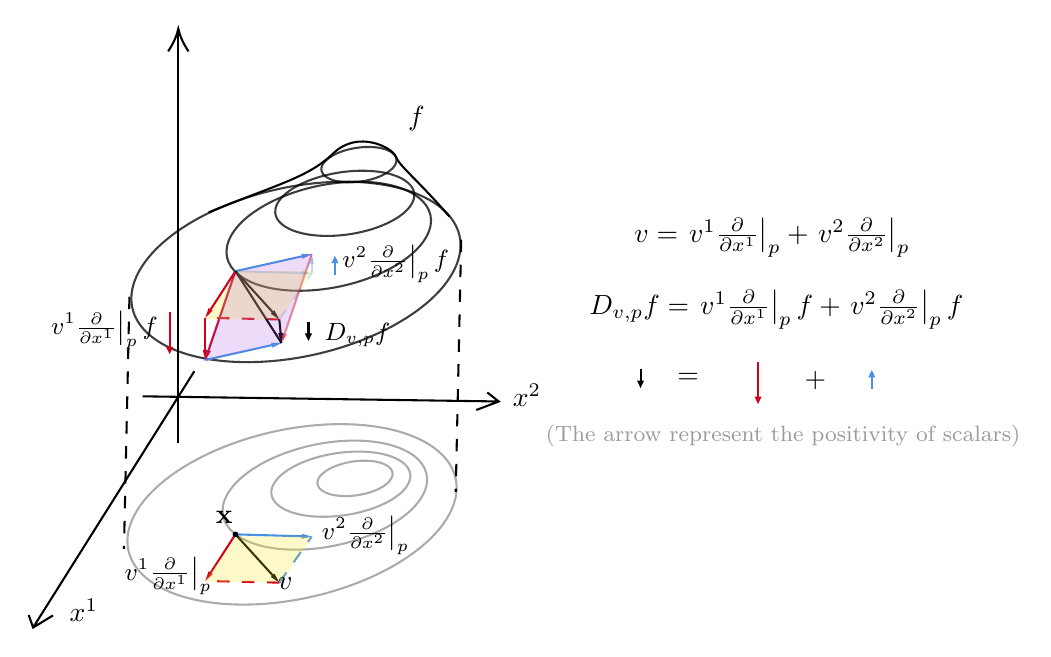
\begin{tikzpicture}[x=0.75pt,y=0.75pt,yscale=-1,xscale=1]
%uncomment if require: \path (0,324); %set diagram left start at 0, and has height of 324

%Shape: Axis 2D [id:dp392022965918875] 
\draw  (233.79,180.44) -- (156.1,303.95)(380.45,195.03) -- (208.86,192.55) (165.68,298.11) -- (156.1,303.95) -- (153.98,297.94) (374.92,190.68) -- (380.45,195.03) -- (369.6,199.15)  ;
%Straight Lines [id:da6093238245580039] 
\draw    (226.05,214.91) -- (226.05,17.44) ;
\draw [shift={(226.05,15.44)}, rotate = 90] [color={rgb, 255:red, 0; green, 0; blue, 0 }  ][line width=0.75]    (10.93,-4.9) .. controls (6.95,-2.3) and (3.31,-0.67) .. (0,0) .. controls (3.31,0.67) and (6.95,2.3) .. (10.93,4.9)   ;
%Shape: Ellipse [id:dp405330952821648] 
\draw  [color={rgb, 255:red, 0; green, 0; blue, 0 }  ,draw opacity=0.33 ][line width=0.75]  (205.09,249.42) .. controls (218.03,225.42) and (262.43,205.96) .. (304.26,205.96) .. controls (346.1,205.96) and (369.52,225.42) .. (356.59,249.42) .. controls (343.65,273.43) and (299.25,292.89) .. (257.41,292.89) .. controls (215.58,292.89) and (192.15,273.43) .. (205.09,249.42) -- cycle ;
%Shape: Ellipse [id:dp329912503849465] 
\draw  [color={rgb, 255:red, 0; green, 0; blue, 0 }  ,draw opacity=0.33 ][line width=0.75]  (249.46,240.15) .. controls (257.28,225.64) and (284.74,213.88) .. (310.81,213.88) .. controls (336.87,213.88) and (351.65,225.64) .. (343.84,240.15) .. controls (336.02,254.66) and (308.55,266.43) .. (282.49,266.43) .. controls (256.43,266.43) and (241.64,254.66) .. (249.46,240.15) -- cycle ;
%Shape: Ellipse [id:dp1514768215459963] 
\draw  [color={rgb, 255:red, 0; green, 0; blue, 0 }  ,draw opacity=0.33 ][line width=0.75]  (271.95,234.87) .. controls (276.62,226.2) and (294.92,219.17) .. (312.82,219.17) .. controls (330.72,219.17) and (341.44,226.2) .. (336.77,234.87) .. controls (332.09,243.54) and (313.79,250.58) .. (295.89,250.58) .. controls (277.99,250.58) and (267.27,243.54) .. (271.95,234.87) -- cycle ;
%Shape: Ellipse [id:dp668836996840452] 
\draw  [color={rgb, 255:red, 0; green, 0; blue, 0 }  ,draw opacity=0.33 ][line width=0.75]  (293.63,232.09) .. controls (296.17,227.38) and (306.09,223.57) .. (315.78,223.57) .. controls (325.48,223.57) and (331.28,227.38) .. (328.75,232.09) .. controls (326.21,236.8) and (316.29,240.62) .. (306.6,240.62) .. controls (296.9,240.62) and (291.1,236.8) .. (293.63,232.09) -- cycle ;
%Shape: Ellipse [id:dp5532471875103369] 
\draw  [color={rgb, 255:red, 0; green, 0; blue, 0 }  ,draw opacity=0.76 ][line width=0.75]  (206.98,132.61) .. controls (219.91,108.61) and (264.31,89.15) .. (306.15,89.15) .. controls (347.98,89.15) and (371.41,108.61) .. (358.47,132.61) .. controls (345.54,156.62) and (301.14,176.08) .. (259.3,176.08) .. controls (217.47,176.08) and (194.04,156.62) .. (206.98,132.61) -- cycle ;
%Shape: Ellipse [id:dp9452353927265793] 
\draw  [color={rgb, 255:red, 0; green, 0; blue, 0 }  ,draw opacity=0.76 ][fill={rgb, 255:red, 255; green, 255; blue, 255 }  ,fill opacity=0 ][line width=0.75]  (251.35,115.42) .. controls (259.17,100.91) and (286.63,89.15) .. (312.69,89.15) .. controls (338.75,89.15) and (353.54,100.91) .. (345.72,115.42) .. controls (337.9,129.93) and (310.44,141.69) .. (284.38,141.69) .. controls (258.32,141.69) and (243.53,129.93) .. (251.35,115.42) -- cycle ;
%Shape: Ellipse [id:dp6430572088651332] 
\draw  [color={rgb, 255:red, 0; green, 0; blue, 0 }  ,draw opacity=0.76 ][line width=0.75]  (273.83,99.57) .. controls (278.51,90.89) and (296.81,83.86) .. (314.71,83.86) .. controls (332.61,83.86) and (343.33,90.89) .. (338.65,99.57) .. controls (333.98,108.24) and (315.68,115.27) .. (297.78,115.27) .. controls (279.88,115.27) and (269.16,108.24) .. (273.83,99.57) -- cycle ;
%Shape: Ellipse [id:dp9802682025318046] 
\draw  [color={rgb, 255:red, 0; green, 0; blue, 0 }  ,draw opacity=0.76 ][line width=0.75]  (295.52,80.94) .. controls (298.06,76.23) and (307.98,72.41) .. (317.67,72.41) .. controls (327.37,72.41) and (333.17,76.23) .. (330.63,80.94) .. controls (328.1,85.64) and (318.18,89.46) .. (308.49,89.46) .. controls (298.79,89.46) and (292.99,85.64) .. (295.52,80.94) -- cycle ;
%Straight Lines [id:da11602801671001872] 
\draw  [dash pattern={on 4.5pt off 4.5pt}]  (202.51,144.58) -- (199.87,266.1) ;
%Straight Lines [id:da3663397544467202] 
\draw  [dash pattern={on 4.5pt off 4.5pt}]  (362.35,117.1) -- (359.71,238.63) ;
%Straight Lines [id:da279639923860469] 
\draw    (253.59,259.06) -- (273.38,280.83) ;
\draw [shift={(274.72,282.31)}, rotate = 227.73] [fill={rgb, 255:red, 0; green, 0; blue, 0 }  ][line width=0.08]  [draw opacity=0] (4.8,-1.2) -- (0,0) -- (4.8,1.2) -- cycle    ;
%Straight Lines [id:da8774565171359308] 
\draw [color={rgb, 255:red, 208; green, 2; blue, 27 }  ,draw opacity=1 ]   (253.59,259.06) -- (240.15,279.84) ;
\draw [shift={(239.06,281.51)}, rotate = 302.91] [fill={rgb, 255:red, 208; green, 2; blue, 27 }  ,fill opacity=1 ][line width=0.08]  [draw opacity=0] (4.8,-1.2) -- (0,0) -- (4.8,1.2) -- cycle    ;
%Straight Lines [id:da8997087652486269] 
\draw [color={rgb, 255:red, 74; green, 144; blue, 226 }  ,draw opacity=1 ]   (253.59,259.06) -- (288.31,260.06) ;
\draw [shift={(290.31,260.12)}, rotate = 181.65] [fill={rgb, 255:red, 74; green, 144; blue, 226 }  ,fill opacity=1 ][line width=0.08]  [draw opacity=0] (4.8,-1.2) -- (0,0) -- (4.8,1.2) -- cycle    ;
%Straight Lines [id:da6154119844672867] 
\draw [color={rgb, 255:red, 208; green, 2; blue, 27 }  ,draw opacity=1 ] [dash pattern={on 4.5pt off 4.5pt}]  (274.72,282.31) -- (239.06,281.51) ;
%Straight Lines [id:da2996342937898313] 
\draw [color={rgb, 255:red, 74; green, 144; blue, 226 }  ,draw opacity=1 ] [dash pattern={on 4.5pt off 4.5pt}]  (274.72,282.31) -- (290.31,260.12) ;
%Straight Lines [id:da1112796770946729] 
\draw    (253.59,132.25) -- (273.38,154.02) ;
\draw [shift={(274.72,155.5)}, rotate = 227.73] [fill={rgb, 255:red, 0; green, 0; blue, 0 }  ][line width=0.08]  [draw opacity=0] (4.8,-1.2) -- (0,0) -- (4.8,1.2) -- cycle    ;
%Straight Lines [id:da886645151103884] 
\draw [color={rgb, 255:red, 208; green, 2; blue, 27 }  ,draw opacity=1 ]   (253.59,132.25) -- (240.15,153.02) ;
\draw [shift={(239.06,154.7)}, rotate = 302.91] [fill={rgb, 255:red, 208; green, 2; blue, 27 }  ,fill opacity=1 ][line width=0.08]  [draw opacity=0] (4.8,-1.2) -- (0,0) -- (4.8,1.2) -- cycle    ;
%Straight Lines [id:da7639376209534354] 
\draw [color={rgb, 255:red, 74; green, 144; blue, 226 }  ,draw opacity=0.31 ]   (253.59,132.25) -- (288.31,133.25) ;
\draw [shift={(290.31,133.3)}, rotate = 181.65] [fill={rgb, 255:red, 74; green, 144; blue, 226 }  ,fill opacity=0.31 ][line width=0.08]  [draw opacity=0] (4.8,-1.2) -- (0,0) -- (4.8,1.2) -- cycle    ;
%Straight Lines [id:da5097974109962886] 
\draw [color={rgb, 255:red, 208; green, 2; blue, 27 }  ,draw opacity=1 ] [dash pattern={on 4.5pt off 4.5pt}]  (274.72,155.5) -- (239.06,154.7) ;
%Straight Lines [id:da5431834208380764] 
\draw [color={rgb, 255:red, 74; green, 144; blue, 226 }  ,draw opacity=0.27 ] [dash pattern={on 4.5pt off 4.5pt}]  (274.72,155.5) -- (290.31,133.3) ;
%Straight Lines [id:da7424431322975342] 
\draw [color={rgb, 255:red, 208; green, 2; blue, 27 }  ,draw opacity=1 ]   (239.06,154.7) -- (239.06,173.05) ;
\draw [shift={(239.06,175.05)}, rotate = 270] [fill={rgb, 255:red, 208; green, 2; blue, 27 }  ,fill opacity=1 ][line width=0.08]  [draw opacity=0] (4.8,-1.2) -- (0,0) -- (4.8,1.2) -- cycle    ;
%Straight Lines [id:da2537352780362212] 
\draw [color={rgb, 255:red, 74; green, 144; blue, 226 }  ,draw opacity=0.35 ]   (290.31,133.3) -- (290.31,126.06) ;
\draw [shift={(290.31,124.06)}, rotate = 90] [fill={rgb, 255:red, 74; green, 144; blue, 226 }  ,fill opacity=0.35 ][line width=0.08]  [draw opacity=0] (4.8,-1.2) -- (0,0) -- (4.8,1.2) -- cycle    ;
%Straight Lines [id:da8538391770378861] 
\draw [color={rgb, 255:red, 208; green, 2; blue, 27 }  ,draw opacity=1 ]   (253.59,132.25) -- (239.7,173.15) ;
\draw [shift={(239.06,175.05)}, rotate = 288.75] [fill={rgb, 255:red, 208; green, 2; blue, 27 }  ,fill opacity=1 ][line width=0.08]  [draw opacity=0] (4.8,-1.2) -- (0,0) -- (4.8,1.2) -- cycle    ;
%Straight Lines [id:da24860430184280746] 
\draw [color={rgb, 255:red, 74; green, 144; blue, 226 }  ,draw opacity=1 ]   (253.59,132.25) -- (288.36,124.49) ;
\draw [shift={(290.31,124.06)}, rotate = 167.43] [fill={rgb, 255:red, 74; green, 144; blue, 226 }  ,fill opacity=1 ][line width=0.08]  [draw opacity=0] (4.8,-1.2) -- (0,0) -- (4.8,1.2) -- cycle    ;
%Straight Lines [id:da25433393648592717] 
\draw [color={rgb, 255:red, 74; green, 144; blue, 226 }  ,draw opacity=1 ]   (239.06,175.05) -- (273.83,167.29) ;
\draw [shift={(275.78,166.86)}, rotate = 167.43] [fill={rgb, 255:red, 74; green, 144; blue, 226 }  ,fill opacity=1 ][line width=0.08]  [draw opacity=0] (4.8,-1.2) -- (0,0) -- (4.8,1.2) -- cycle    ;
%Straight Lines [id:da2651028764912726] 
\draw [color={rgb, 255:red, 208; green, 2; blue, 27 }  ,draw opacity=0.45 ]   (290.31,124.06) -- (276.42,164.96) ;
\draw [shift={(275.78,166.86)}, rotate = 288.75] [fill={rgb, 255:red, 208; green, 2; blue, 27 }  ,fill opacity=0.45 ][line width=0.08]  [draw opacity=0] (4.8,-1.2) -- (0,0) -- (4.8,1.2) -- cycle    ;
%Straight Lines [id:da887357681214503] 
\draw    (274.72,155.5) -- (275.6,164.86) ;
\draw [shift={(275.78,166.86)}, rotate = 264.69] [fill={rgb, 255:red, 0; green, 0; blue, 0 }  ][line width=0.08]  [draw opacity=0] (4.8,-1.2) -- (0,0) -- (4.8,1.2) -- cycle    ;
%Straight Lines [id:da9879518755298273] 
\draw    (253.59,132.25) -- (275.78,166.86) ;
%Shape: Rectangle [id:dp48139861566876485] 
\draw  [color={rgb, 255:red, 0; green, 0; blue, 0 }  ,draw opacity=0 ][fill={rgb, 255:red, 248; green, 231; blue, 28 }  ,fill opacity=0.24 ] (254.91,132.25) -- (290.58,132.25) -- (274.72,155.5) -- (239.06,155.5) -- cycle ;
%Shape: Rectangle [id:dp228264440355205] 
\draw  [color={rgb, 255:red, 0; green, 0; blue, 0 }  ,draw opacity=0 ][fill={rgb, 255:red, 165; green, 80; blue, 227 }  ,fill opacity=0.2 ] (252.85,132.87) -- (290.74,123.52) -- (275.71,166.44) -- (237.82,175.79) -- cycle ;
%Shape: Rectangle [id:dp7530585387976709] 
\draw  [color={rgb, 255:red, 0; green, 0; blue, 0 }  ,draw opacity=0 ][fill={rgb, 255:red, 248; green, 231; blue, 28 }  ,fill opacity=0.24 ] (253.96,260.12) -- (290.75,260.12) -- (275.39,282.04) -- (238.6,282.04) -- cycle ;
%Shape: Ellipse [id:dp5682659762825244] 
\draw  [color={rgb, 255:red, 0; green, 0; blue, 0 }  ,draw opacity=0 ][fill={rgb, 255:red, 0; green, 0; blue, 0 }  ,fill opacity=1 ] (252.18,259.06) .. controls (252.18,258.31) and (252.81,257.7) .. (253.59,257.7) .. controls (254.37,257.7) and (254.99,258.31) .. (254.99,259.06) .. controls (254.99,259.81) and (254.37,260.42) .. (253.59,260.42) .. controls (252.81,260.42) and (252.18,259.81) .. (252.18,259.06) -- cycle ;
%Curve Lines [id:da2976014961647424] 
\draw    (240.67,103.93) .. controls (273.87,90.33) and (288.67,87.13) .. (300.67,75.53) .. controls (312.67,63.93) and (329.27,72.73) .. (330.87,77.13) .. controls (332.47,81.53) and (341.87,88.73) .. (356.67,105.93) ;
%Straight Lines [id:da10174581755467726] 
\draw [color={rgb, 255:red, 208; green, 2; blue, 27 }  ,draw opacity=1 ]   (221.86,151.9) -- (221.86,169.25) ;
\draw [shift={(221.86,172.25)}, rotate = 270] [fill={rgb, 255:red, 208; green, 2; blue, 27 }  ,fill opacity=1 ][line width=0.08]  [draw opacity=0] (3.57,-1.72) -- (0,0) -- (3.57,1.72) -- cycle    ;
%Straight Lines [id:da8263939691535676] 
\draw [color={rgb, 255:red, 74; green, 144; blue, 226 }  ,draw opacity=1 ]   (301.51,134.1) -- (301.51,127.86) ;
\draw [shift={(301.51,124.86)}, rotate = 90] [fill={rgb, 255:red, 74; green, 144; blue, 226 }  ,fill opacity=1 ][line width=0.08]  [draw opacity=0] (3.57,-1.72) -- (0,0) -- (3.57,1.72) -- cycle    ;
%Straight Lines [id:da6821225686661974] 
\draw [color={rgb, 255:red, 0; green, 0; blue, 0 }  ,draw opacity=1 ]   (288.76,162.85) -- (288.76,156.61) ;
\draw [shift={(288.76,165.85)}, rotate = 270] [fill={rgb, 255:red, 0; green, 0; blue, 0 }  ,fill opacity=1 ][line width=0.08]  [draw opacity=0] (3.57,-1.72) -- (0,0) -- (3.57,1.72) -- cycle    ;
%Straight Lines [id:da420763728946844] 
\draw [color={rgb, 255:red, 208; green, 2; blue, 27 }  ,draw opacity=1 ]   (505.36,175.9) -- (505.36,193.25) ;
\draw [shift={(505.36,196.25)}, rotate = 270] [fill={rgb, 255:red, 208; green, 2; blue, 27 }  ,fill opacity=1 ][line width=0.08]  [draw opacity=0] (3.57,-1.72) -- (0,0) -- (3.57,1.72) -- cycle    ;
%Straight Lines [id:da7927683614331424] 
\draw [color={rgb, 255:red, 74; green, 144; blue, 226 }  ,draw opacity=1 ]   (560.18,189.1) -- (560.18,182.86) ;
\draw [shift={(560.18,179.86)}, rotate = 90] [fill={rgb, 255:red, 74; green, 144; blue, 226 }  ,fill opacity=1 ][line width=0.08]  [draw opacity=0] (3.57,-1.72) -- (0,0) -- (3.57,1.72) -- cycle    ;
%Straight Lines [id:da1481174141229029] 
\draw [color={rgb, 255:red, 0; green, 0; blue, 0 }  ,draw opacity=1 ]   (448.76,185.52) -- (448.76,179.27) ;
\draw [shift={(448.76,188.52)}, rotate = 270] [fill={rgb, 255:red, 0; green, 0; blue, 0 }  ,fill opacity=1 ][line width=0.08]  [draw opacity=0] (3.57,-1.72) -- (0,0) -- (3.57,1.72) -- cycle    ;

% Text Node
\draw (172.25,288.57) node [anchor=north west][inner sep=0.75pt]    {$x^{1}$};
% Text Node
\draw (385.75,185.15) node [anchor=north west][inner sep=0.75pt]    {$x^{2}$};
% Text Node
\draw (272.67,278.15) node [anchor=north west][inner sep=0.75pt]    {$\bm{v}$};
% Text Node
\draw (292.17,248.95) node [anchor=north west][inner sep=0.75pt]  [font=\small]  {${\textstyle \left. v^{2}\frac{\partial }{\partial x^{2}}\right| _{p}}$};
% Text Node
\draw (197.06,268.56) node [anchor=north west][inner sep=0.75pt]  [font=\small]  {${\textstyle \left. v^{1}\frac{\partial }{\partial x^{1}}\right| _{p}}$};
% Text Node
\draw (242.65,246.19) node [anchor=north west][inner sep=0.75pt]    {${\textstyle \mathbf{x}}$};
% Text Node
\draw (161.66,150.21) node [anchor=north west][inner sep=0.75pt]  [font=\small]  {${\textstyle \left. v^{1}\frac{\partial }{\partial x^{1}}\right| _{p} f}$};
% Text Node
\draw (302.06,118.21) node [anchor=north west][inner sep=0.75pt]  [font=\small]  {${\textstyle \left. v^{2}\frac{\partial }{\partial x^{2}}\right| _{p} f}$};
% Text Node
\draw (295.08,155.71) node [anchor=north west][inner sep=0.75pt]  [font=\small]  {$D_{v,p} f$};
% Text Node
\draw (444.33,105.13) node [anchor=north west][inner sep=0.75pt]  [font=\normalsize]  {$\bm{v} ={\textstyle \left. v^{1}\frac{\partial }{\partial x^{1}}\right| _{p} +\left. v^{2}\frac{\partial }{\partial x^{2}}\right| _{p}}$};
% Text Node
\draw (422.62,139.91) node [anchor=north west][inner sep=0.75pt]  [font=\normalsize]  {$D_{v,p} f={\textstyle \left. v^{1}\frac{\partial }{\partial x^{1}}\right| _{p} f+\left. v^{2}\frac{\partial }{\partial x^{2}}\right| _{p} f}$};
% Text Node
\draw (335.33,51.4) node [anchor=north west][inner sep=0.75pt]    {$f$};
% Text Node
\draw (465,180.07) node [anchor=north west][inner sep=0.75pt]    {$=$};
% Text Node
\draw (526.33,179.13) node [anchor=north west][inner sep=0.75pt]    {$+$};
% Text Node
\draw (401.67,204.89) node [anchor=north west][inner sep=0.75pt]  [font=\footnotesize,color={rgb, 255:red, 155; green, 155; blue, 155 }  ,opacity=1 ] [align=left] {(The arrow represent the positivity of scalars)};


\end{tikzpicture}
